%%%%%%%%%%%%%%%%%%%%%%%%%%%%%%%%%%%%%%%%%
% fphw Assignment
% LaTeX Template
% Version 1.0 (27/04/2019)
%
% This template originates from:
% https://www.LaTeXTemplates.com
%
% Authors:
% Class by Felipe Portales-Oliva (f.portales.oliva@gmail.com) with template 
% content and modifications by Vel (vel@LaTeXTemplates.com)
%
% Template (this file) License:
% CC BY-NC-SA 3.0 (http://creativecommons.org/licenses/by-nc-sa/3.0/)
%
%%%%%%%%%%%%%%%%%%%%%%%%%%%%%%%%%%%%%%%%%

%----------------------------------------------------------------------------------------
%	PACKAGES AND OTHER DOCUMENT CONFIGURATIONS
%----------------------------------------------------------------------------------------

\documentclass[
	12pt, % Default font size, values between 10pt-12pt are allowed
	%letterpaper, % Uncomment for US letter paper size
	%spanish, % Uncomment for Spanish
]{fphw}

% Template-specific packages
\usepackage[utf8]{inputenc} % Required for inputting international characters
\usepackage[T1]{fontenc} % Output font encoding for international characters
\usepackage{mathpazo} % Use the Palatino font

\usepackage{graphicx} % Required for including images

\usepackage{booktabs} % Required for better horizontal rules in tables

\usepackage{listings} % Required for insertion of code

\usepackage{enumerate} % To modify the enumerate environment

\usepackage{leadsheets}

\usepackage{xcolor}

\usepackage{float}

%----------------------------------------------------------------------------------------
%	ASSIGNMENT INFORMATION
%----------------------------------------------------------------------------------------

\title{Homework \#2 - Template-Based Chord Recognition} % Assignment title

\author{Matteo Pettenò - Marco Viviani} % Students name

\date{December 23th, 2021} % Due date

\institute{Politecnico di Milano} % Institute or school name

\class{Computer Music - Representations and Models} % Course or class name

\professor{Clara Borrelli} % Professor or teacher in charge of the assignment

%----------------------------------------------------------------------------------------

\begin{document}

\maketitle % Output the assignment title, created automatically using the information in the custom commands above

%----------------------------------------------------------------------------------------
%	ASSIGNMENT CONTENT
%----------------------------------------------------------------------------------------

\section*{Question 1}

\begin{problem}
	Implement the template based chord recognition algorithm.
\end{problem}

\subsection*{Answer}

The aim of this homework is to implement the template based chord recognition algorithm. For doing this, we define a function that takes as input the path to a .wav file and returns the estimated chords sequence labels:

\begin{lstlisting}
def compute_template_based_chord_recognition(audio_file_path)
\end{lstlisting}

The output is a list where each element is the predicted chord label for the time frame n.

A chord recognition algorithm consists of two steps. In the first step, the given audio recording is cut into frames that are transformed into a feature vector. This is tipically done with chroma-based audio features, which contain the tonal information of the audio signal.
In the second step, pattern matching techniques are used to map each feature vector to a set of predefined chord models. The best fit determines the chord label assigned to the given frame.

\subsection{Import}
In the first cell we import all the libraries needed for the implementation of the code. Among them we can notice \textit{copy, re, librosa, pandas} and \textit{libfmp.b}.

\subsection{Context initialization}
In this section we decided to initialize a dictionary with song library details (experiment corpus) in order to have a code that is easier to read. In this way it will also be easier to change the parameters (question 5), doing it directly from this cell.

\subsection{Parameters configuration}
This section of the code establishes all the known parameters and values that will be used to develop the code. It will be possible to change the parameters directly from this section when needed (question 5).

\subsection{Features processing functions}
In this section of the code all the functions that will be useful to implement features processing are defined. To improve the chord recognition results, in fact, additional enhancement techniques are applied either before the pattern matching step (referred to as prefiltering) or after/within the pattern matching step (referred to as postfiltering).

\subsubsection{Pre-filtering}

\begin{lstlisting}
1) def compress_feature_sequence(feature_sequence, gamma = 0.1)
\end{lstlisting}
This function takes in input the sequence of features and applies compression in a logarithmic fashion.
\begin{lstlisting}
2) def normalize_feature_sequence(feature_sequence, norm='2', v=None)
\end{lstlisting}
This function normalizes the columns of a feature sequence. One normalization strategy is to choose a suitable norm  and then to replace each n-feature vector  by $ x/p(x) $.
The normalization procedure as described above replaces each chroma vector by its normalized version. Intuitively speaking, normalization introduces a kind of invariance to differences in dynamics or sound intensity.
The normalization procedure is only possible if $p(x) \neq 0
$. Also for very small values $p(x)$ which may occur in passages of silence before the actual start of the recording or during long pauses, normalization would lead to more or less random and therefore meaningless chroma value distributions. Therefore, if $p(x)$ calls below a certain threshold, the vector $x$ may be replaced by some standard vector such as a uniform vector of norm one instead of dividing by $p(x)$. In the function exactly this steps are implemented.
Normalization will be used also in post filtering in order to normalize the chord similarities.

\subsubsection{Post-filtering}

\begin{lstlisting}
1) def smooth_feature_sequence(feature_sequence)
\end{lstlisting}
For certain music retrieval applications, chromagrams may be too detailed. In particular, it may be desirable to further increase the similarity between them. This can be achieved by smoothing procedures applied in a postprocessing step. The idea is to compute for each chroma dimension a kind of local average over time.
More precisely, let $X=(x(1),x(2),...,x(N))$ be a feature sequence with $x(n)\in \mathbb{R}^k$ for $\in$[1:N], and let be $w$ a rectangular window  of length L. Then we compute for each $k \in$ [1:N] a convolution between $w$ and the sequence $[x1(k),x2(k),...,xN(k)]$. Assuming a centered view, we only keep the center part of length of the convolution (\textit{scipy.signal.convolve}). The result is a smoothed feature sequence of the same dimensions.
For the window (also called kernel) results in a bandwise 1D convolution. Using the parameter mode='same' enforces the centered view. As for the window , one may also use other window types such as a Hann window.
Applying temporal smoothing using a rectangular or a Hann window can be regarded as bandwise lowpass filtering, which attenuates fast temporal fluctuations in the feature representation.

\begin{lstlisting}
2) def downsample_feature_sequence(feature_sequence, feature_rate)
\end{lstlisting}

Often, to increase the efficiency of subsequent processing and analysis steps, one decimates the smoothed representation by keeping only every D-th feature, where D$\in\mathbb{N}$ is a suitable constant (typically much smaller than the window length L). This decimation, which is also referred to as downsampling, reduces the feature rate by a factor D.

\subsection{Template-based chord recognition steps and functions}
In this cell of the code are defined all the function that will be used in order to compute the chord recognition steps:
\begin{lstlisting}
1) def load_audio(wav_file_path: str)
\end{lstlisting}
Loads the .wav file.
\begin{lstlisting}
2) def chroma_representation(audio_file)
\end{lstlisting}
Computes chroma features with STFT to the eventually compressed features.
\begin{lstlisting}
3) def generate_triads_templates()
\end{lstlisting}
Generate chord templates of major and minor triads. This function takes no input and returns the matrix containing the chord templates as columns.
Every column will be a binary vector representing the template for every minor or major chord.
\begin{lstlisting}
4) def generate_chord_labels()
\end{lstlisting}
Generate a chord labels list for major and minor triads.
This function takes no inputs and generates a list where major chords are indicated only with the tonic note and minor chords with the tonic note plus the simbol "m" (minor).
\begin{lstlisting}
5) def pre_processing(chroma_features, chroma_feature_rate, triads_templates)
\end{lstlisting}
The aim of this function is to pre-process the features used in the algorithm.
With the previous defined functions it normalizes, smooths and downsamples chroma features and triads template.
\begin{lstlisting}
6) def pattern_matching(chroma_features, triads_template)
\end{lstlisting}
It computes the \textit{similarity measure} (\textit{np.matmul}) between the triads template models and the predicted chroma features,according to this formula $(x,y)=\langle x,y\rangle/(||x||*||y||)$.

\begin{lstlisting}
7) def post_processing(chord_similarity)
\end{lstlisting}
In this section is applied post-processing through normalization to chord similarity, in order to have normalized results.
\begin{lstlisting}
8) def recognition_result(chord_similarity, triads_templates)
\end{lstlisting}
This function takes as input the matrix of triads templates and compares the current chord with the various templates. The tamplate of the chord that maximizes the chord similarity is the correct one.\\
VEDI MEGLIO

\subsection{Template-based chord recognition implementation}

While the previous cells contain the function useful to the code, in this section there is the function that implements the real algorithm:\\

\begin{lstlisting}
def compute_template_based_chord_recognition(audio_file_path)
\end{lstlisting}
In first place, the function loads the audio file.\\ After that, it computes chromagram where, as said before, is performed pre-processing through compression. It is also necessary to create the triads template that is useful to compare with the predicted chord.\\
As said before is necessary to apply pre-processing with the previously defined function (normalization, smoothing, downsampling).
Then, we have to compare the predicted chord through pattern matching and post-process the result.
Only at the end we can recognize the chord through maximum similarity principle.\\

\begin{figure}[H]
 \centering
 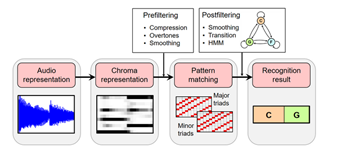
\includegraphics[scale=1]{./images/1_template_based_pipeline.png}
 \caption{Template-Based Chord Recognition Pipeline}
\end{figure}

\subsection{Perform template-based chord recognition and plot results}

In this last section we perform the algorithm with the main function previous defined with the song "Beatles LetItBe.wav". This last part of the code plots the audio signal, the chromagram, the  similarity matrix and chord recognition results.\\

\begin{figure}[H]
 \centering
 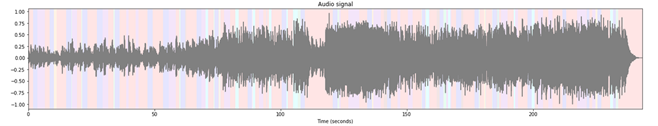
\includegraphics[scale=1]{./images/1_audio_signal.png}
 \caption{Audio Signal}
\end{figure}

\begin{figure}[H]
 \centering
 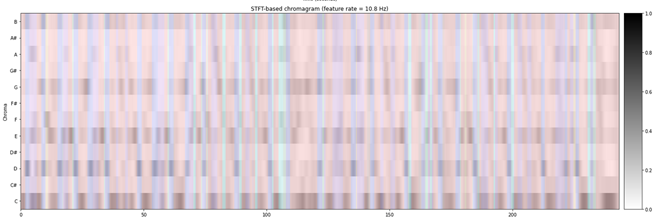
\includegraphics[scale=1]{./images/1_stft_chromagram.png}
 \caption{STFT-based Chromagram}
\end{figure}

\begin{figure}[H]
 \centering
 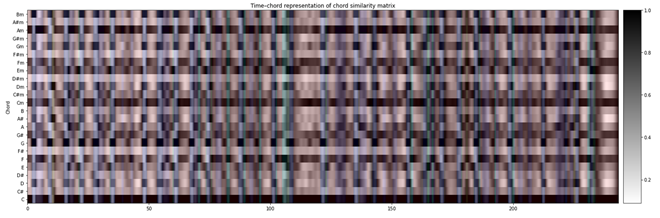
\includegraphics[scale=1]{./images/1_chord_similarity.png}
 \caption{Chord Similarity Matrix}
\end{figure}

\begin{figure}[H]
 \centering
 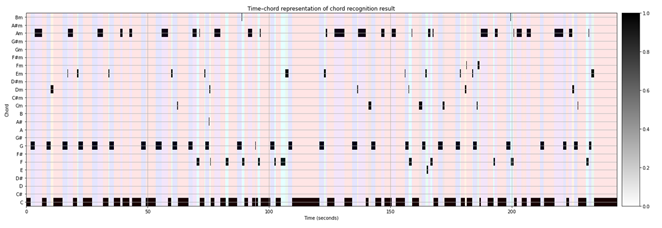
\includegraphics[scale=1]{./images/1_recognition_results.png}
 \caption{Chord Recognition Results}
\end{figure}

%----------------------------------------------------------------------------------------

\section*{Question 2}

\begin{problem}
	Write a function to load and preprocess a reference annotation (or ground truth) file, saved in CSV
format.
\end{problem}

\subsection*{Answer}

In this section is asked to write a function to load and preprocess a reference annotation (or ground truth) file, saved in CSV:\\

\begin{lstlisting}
def read_ground_truth(csv_file_path)
\end{lstlisting}


The function should take as input the path to a CSV file and produce as output a list of ground truth chord labels, after suitable pre processing.\\
The output must be a list where each element
n is the ground truth chord label for the n-th time window.

\subsection{Ground truth processing functions - Pre-processing phase}
In this paragraph is explaied each step of the preprocessing phase, focusing in particular on the reduction strategy of the chord label set.
\begin{lstlisting}
def read_csv(csv_file_path)
\end{lstlisting}
Reads the path of the .csv file.
\begin{lstlisting}
def convert_segment_annotations(segment_annotation_indices)
\end{lstlisting}
The function (required in the first point, question 2) has the important role to convert the segment-based annotation into a frame-based label sequence adapted to the feature rate used for the chroma sequence.\\

\begin{lstlisting}
def get_binary_time_chord_matrix(labels_sequence)
\end{lstlisting}
The function takes as input the sequence of lables and returns the matrix with the duration (in binary rapresentation) of the various chords. It converts the labels used in the annotation file to match the chord labels used for the chord recognition
algorithm in terms of enharmonic equivalence (i.e., Db = C\# ).
VEDI MEGLIO

\begin{lstlisting}
def normalize_chord_labels(chord_labels)
\end{lstlisting}

Important to notice is the function that normalizes chord labels.
It replaces for segment-based annotation in each chord label the string ':min' by 'm' and convert flat chords into sharp chords using enharmonic equivalence. We can also see that half diminished, diminished and minor chords are classified as minor chords with the letter 'm'. Maj, sus and slash  chords are classified as major chords (' '). This is done by using Python's \textit{regex} (regular expressions). In this way we implemented the reduction strategy of the chord label set.


\subsection{Ground truth reading implementation}
The role of this function is to load and preprocess a reference annotation (or ground truth) file, saved in CSV format. The function should takes as input the path to a CSV file and produce as output a list of ground truth chord labels, after suitable pre processing. The output is a list where each n-th element is the ground truth chord label for the time window n.

\begin{lstlisting}
def read_ground_truth(csv_file_path)
\end{lstlisting}

The function converts segment-based chord annotation into various formats and returns a frame by frame reference chords label sequence, the binary time-chord matrix representation of the reference chords label sequence,the original reference annotations given in seconds, the normalized reference annotations given in seconds.


\subsection{Perform ground truth reading}
In this section the code performs ground truth reading, plotting the results of chord recognition.

\begin{figure}[H]
 \centering
 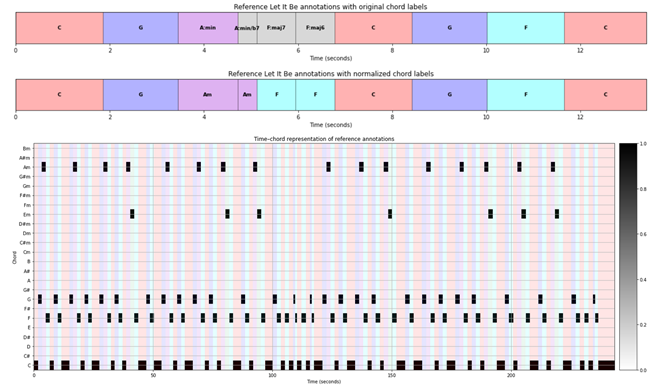
\includegraphics[scale=1]{./images/2_reference_annotations.png}
\end{figure}

%----------------------------------------------------------------------------------------

\section*{Question 3}

\begin{problem}
	Propose a metric for evaluating the template based chord recognition algorithm.
\end{problem}

\subsection*{Answer}

In this section we define a function that takes as input the list of predicted chord labels, the list of ground truth chord labels and computes the proposed metric value.
\begin{lstlisting}
def compute_eval_measures(chord_max, ground_truth_matrix)
\end{lstlisting}
A metric is a scalar number that expresses how good is the algorithm in performing the task of chord recognition.\\

We now introduce a simple evaluation measure. Recall that, given a chroma sequence \(X=(x1,x2,…,xN)\) and a set \( \Lambda :=[C,C\#,…,B,Cm,Cm\#,…,Bm] \)\\

In the context of music structure analysis, we introduce evaluation measures that are used in general information retrieval. We now adapt these notions to our chord recognition scenario. First, we define the set of items to be \(L=[1:N]×\Lambda\). In particular, the non-chord label N is left unconsidered. Then:
\[LRef+:={(n,\lambda Refn) \in L:n\in[1:N]}\]

are the positive (or relevant items) and

\[LEst+:={(n,\lambda n) \in L:n\in[1:N]}\]

are the items estimated as positive (or retrieved items). With these notions, an item (n,$\lambda$n) is called a true positive (TP) in the case that the label is correct (i.e., $\lambda$n=$\lambda$Refn). Otherwise, (n,$\lambda$n) is called a false positive (FP) and (n,$\lambda$Refn) a false negative (FN). All other items in I are called true negative. With these notions, one can define the standard precision (P), recall (R), and F-measure (F):

\[P=(\#TP)/(\#TP + \#FP)\]
\[R=(\#TP)/(\#TP + \#FN)\]
\[P=(2PR)/(P + R)\]

In the way we have formulated our chord recognition problem so far, we have exactly one label per frame in the reference as well as in the estimation. From this follows that \#FP=\#FN and that the definition of accuracy coincides with precision, recall, and F-measure. This is why in the function we use as measure the precision P.

\subsection{Metric evaluation implementation}
\begin{lstlisting}
def compute_eval_measures(chord_max, ground_truth_matrix):
\end{lstlisting}
This function implements exactly the precision measure as said in the previous paragraph.

\subsection{Perform metric evaluation}
\begin{lstlisting}
recognition_precision = compute_eval_measures(chord_max, ground_truth_matrix)
\end{lstlisting}

Computes evaluation for the song "Let it be" by Beatles.\\

\begin{figure}[H]
 \centering
 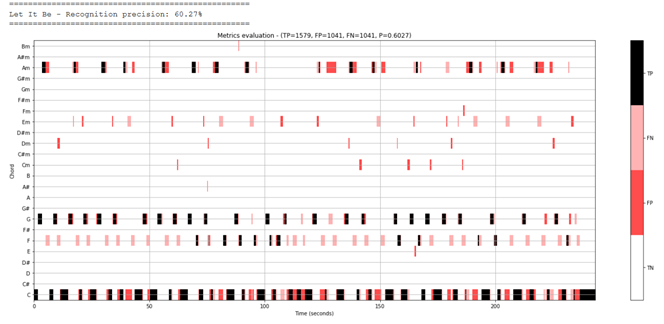
\includegraphics[scale=1]{./images/3_let_it_be_metrics.png}
 \caption{Let It Be - Metrics Evaluation}
\end{figure}

\begin{problem}
	Can you imagine a musically informed strategy that weights diferently mismatch errors of
the chord recognition algorithm?
\end{problem}

%----------------------------------------------------------------------------------------

\section*{Question 4}

\begin{problem}
	Compute the proposed metric for the remaining 3 songs
\end{problem}

\subsection*{Answer}

We compute the proposed metric for the remaining 3 songs:

\begin{figure}[H]
 \centering
 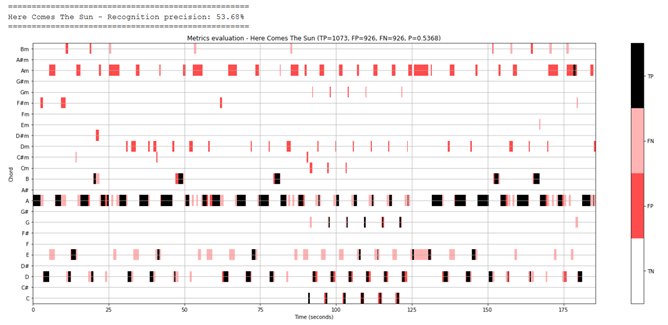
\includegraphics[scale=1]{./images/4_here_comes_the_sun_metrics.png}
 \caption{Here comes the sun}
\end{figure}

\begin{figure}[H]
 \centering
 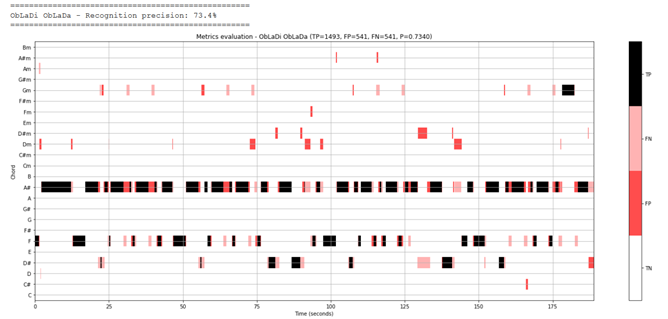
\includegraphics[scale=1]{./images/4_obladi_oblada_metrics.png}
 \caption{ObLaDì ObLada}
\end{figure}

\begin{figure}[H]
 \centering
 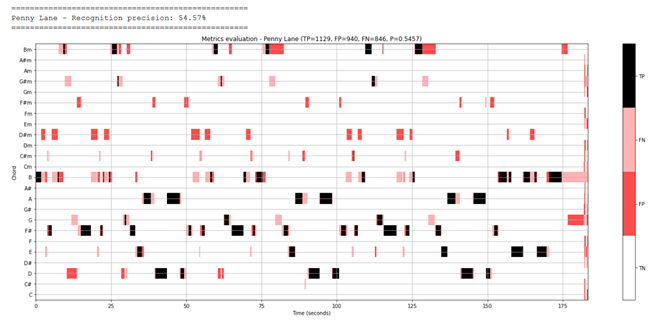
\includegraphics[scale=1]{./images/4_penny_lane_metrics.png}
 \caption{Penny Lane}
\end{figure}

%----------------------------------------------------------------------------------------

\section*{Question 5}

\begin{problem}
	Analyse how algorithm parameters affect the performance of the templated based chord recognition
algorithm.
\end{problem}


\subsection*{Answer}

\subsection{Smooth filter length} 
Applying temporal smoothing using a rectangular or a Hann window can be regarded as bandwise lowpass filtering, which attenuates fast temporal fluctuations in the feature representation. This allows the chord estimation to be much more precise and not be affected by high frequencies. \\

We consider the following vector of values [0,30,60]: we can see an increase in accuracy up to 30 and then a substantial settlement with a slight decrease. The graphs have similar trends.\\

We can deduce that around the value 30 the precision of our algorithm will be higher. However, it is not particularly high. To do this it will also be necessary to observe which are the best values for the other parameters that the algorithm is using. \\

\begin{figure}[H]
 \centering
 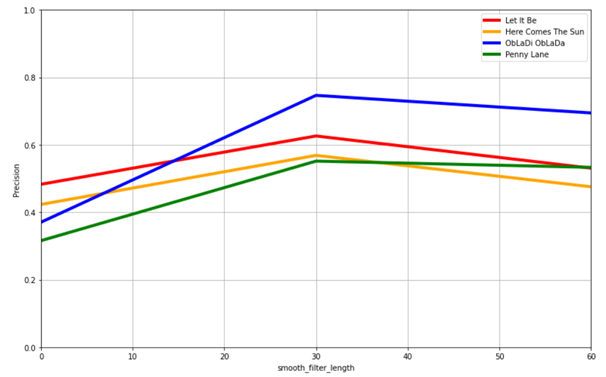
\includegraphics[scale=1]{./images/5_smooth_precision.png}
 \caption{Smooth filter length}
\end{figure}

\subsection{Down sampling factor}
Often, after considering the smooth filter length, to increase the efficiency of subsequent processing and analysis steps, one decimates the smoothed representation by keeping only every H-th feature, where  \(H \in N\) is a suitable constant (typically much smaller than the window length L). This decimation, which is also referred to as downsampling, reduces the feature rate by a factor H.\\

We take into account these values: [0, 10, 100]: the more the downsampling factor is increased, the more you reduce the feature rate and the less you read the harmonic content (in larger steps). If chosen high, inconsistently with the window length, the precision decreases.
It's good to use it in combination with the smoothing filter for efficiency. In this case 10 or less can be a good value. 

\begin{figure}[H]
 \centering
 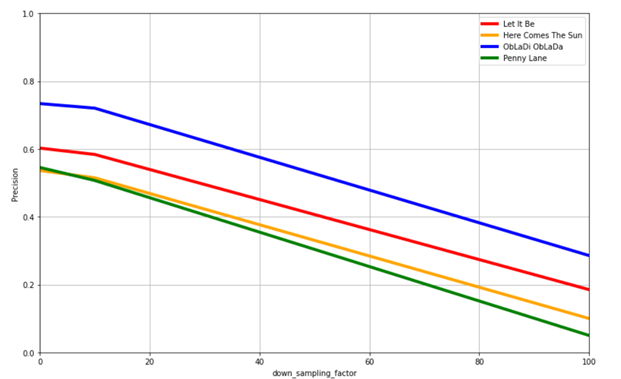
\includegraphics[scale=1]{./images/5_down_sampling_precision.png}
 \caption{Down sampling factor}
\end{figure}

\subsection{Window length}
We consider the following vector of values of window lengths [2048, 8192, 32768]:  using an analysis window with a short duration , each chroma frame contains the onsets of at most one note. Even though the sound of each note may last much longer than the notated duration, the harmonic content of each frame is dominated by only one or two notes. This explains the misclassifications and many chord label changes in the recognition result of the first setting. \\
An obvious strategy for improving the chord recognition result is to use larger window sizes. Anyway, the larger analysis windows smooth out the originally sharp transitions between different chords, which may introduce problems at chord changes.\\

\begin{figure}[H]
 \centering
 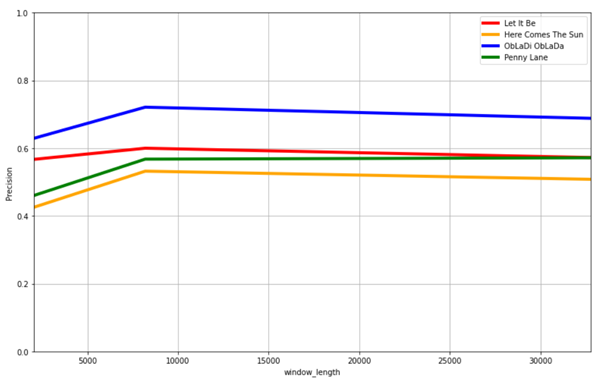
\includegraphics[scale=1]{./images/5_window_precision.png}
 \caption{Window length}
\end{figure}

%----------------------------------------------------------------------------------------

\end{document}
